\section{Data design}

The database contains two tables (\autoref{fig:er}) that are defined by the Prisma Schema. From this schema, Prisma creates a typed Client and an SQL migration for every modification. Each \texttt{User} will contain an ID, email address (unique and converted to all lower-case characters), name, bcrypt password hash and creation time. \autoref{tab:match-table} describes the \texttt{Match} table.

\begin{figure}[H]
	\centering
	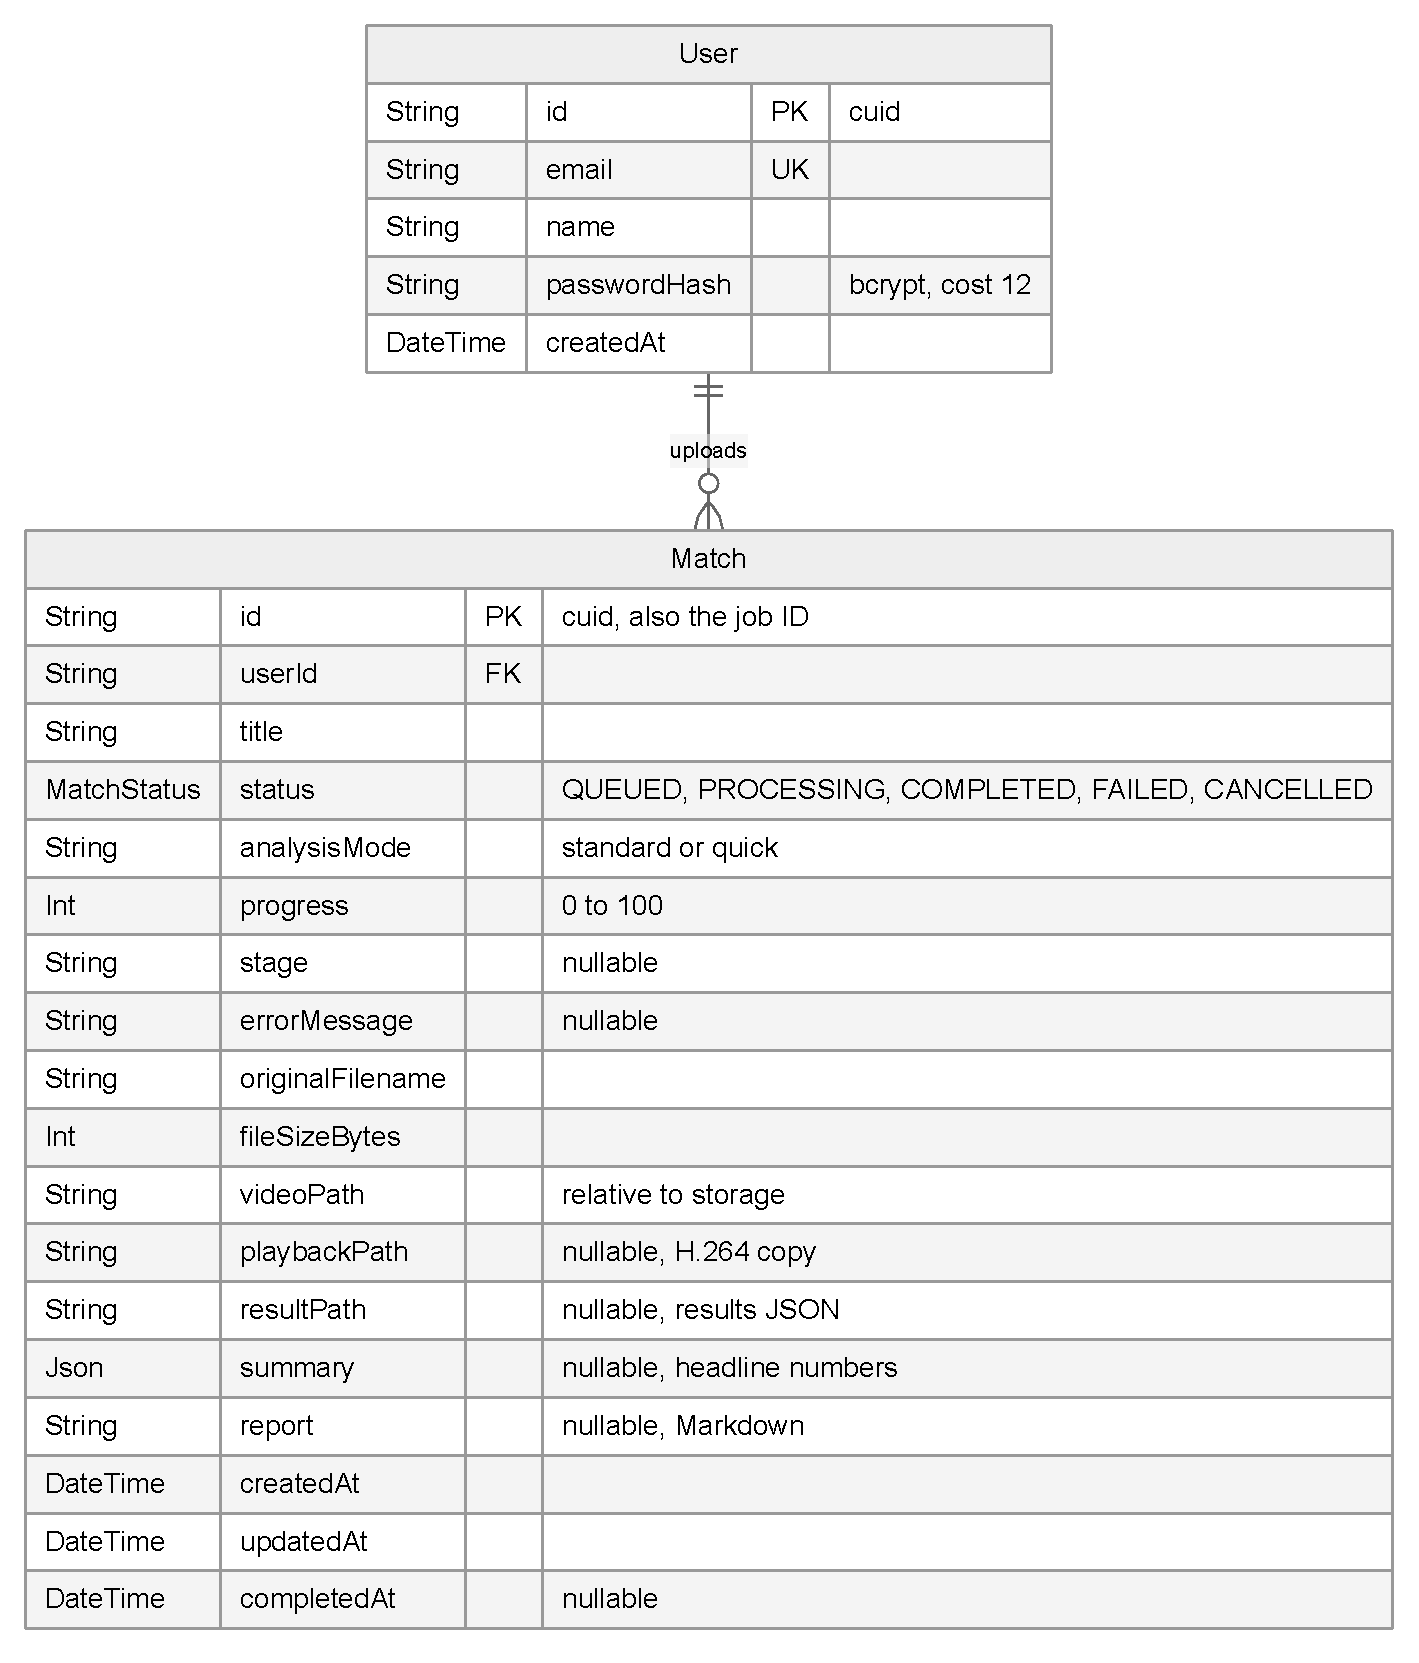
\includegraphics[width=\textwidth]{er}
	\caption{Entity-relationship diagram}
	\label{fig:er}
\end{figure}

\begin{table}[H]
	\centering
	\begin{tabular}{|p{0.24\textwidth}|p{0.67\textwidth}|}
		\hline
		\textbf{Column} & \textbf{Description} \\
		\hline
		id & Unique ID; also the ID of the queue job, so queue events map straight to rows. \\
		\hline
		userId & Owner; deleting a user deletes their matches. \\
		\hline
		title, analysisMode & Title, and \texttt{standard} or \texttt{quick}. \\
		\hline
		status, progress, stage & State (\autoref{fig:status}), 0--100 and the current step. \\
		\hline
		errorMessage & Reason of the last failure. \\
		\hline
		videoPath, playbackPath, resultPath & The upload, its browser-playable copy and the results file, relative to the storage folder. \\
		\hline
		summary & Headline numbers (JSON) for lists and the summary tab. \\
		\hline
		report & The AI coaching report (Markdown). \\
		\hline
		createdAt, completedAt & Creation and completion time. \\
		\hline
	\end{tabular}
	\caption{The \texttt{Match} table}
	\label{tab:match-table}
\end{table}

\begin{figure}[H]
	\centering
	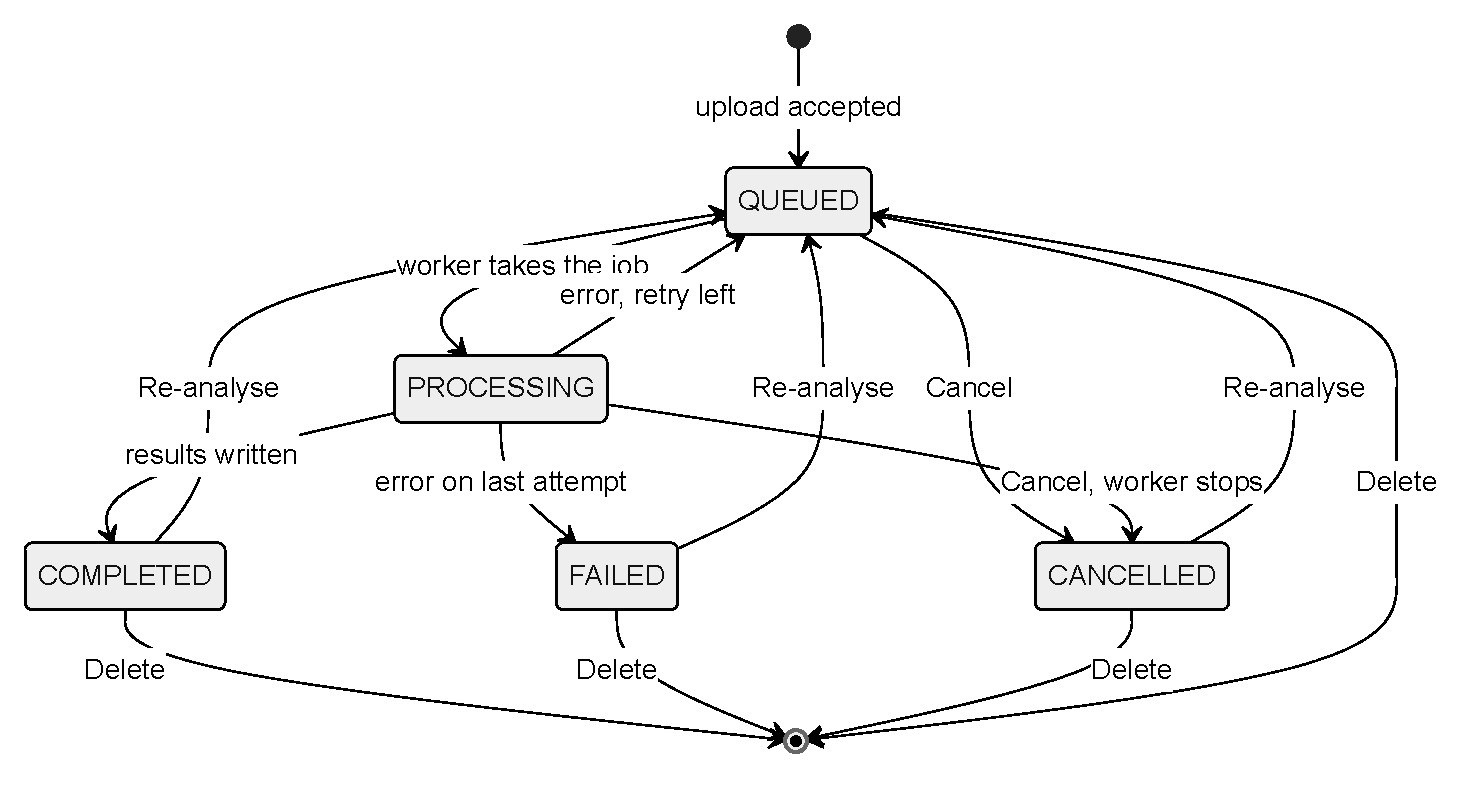
\includegraphics[width=\textwidth]{status}
	\caption{States of a match}
	\label{fig:status}
\end{figure}

The large analysis result files have been intentionally excluded from the database; it would be too much to store every single result in the database (each half generates a 54\,MB results file), but since the results file is stored on the hard drive, the API can serve it from there. Database holds only the small summary. The results file is the contract between the worker and the dashboard (\autoref{tab:results}). A person is represented as a compact array (as opposed to an object) resulting in a smaller file.

\begin{table}[H]
	\centering
	\begin{tabular}{|p{0.2\textwidth}|p{0.7\textwidth}|}
		\hline
		\textbf{Field} & \textbf{Content} \\
		\hline
		video & Frame rate, size, length, and which frames were analysed. \\
		\hline
		teams & Kit colour of each team and the goal it defends. \\
		\hline
		frames & For every analysed frame: each person (track ID, team, role, box, pitch position, position label), the ball, and the camera matrix of the frame. \\
		\hline
		players & For every position of a team: label (e.g. LB), time visible, distance, average and top speed, heatmap. \\
		\hline
		teamShape & Per frame and team: area, width and depth of the outfield players. \\
		\hline
		heatmaps & Where Team A, Team B and the ball spent their time. \\
		\hline
		formations & The formation, runner-up and cost of each team in every 5-second window, and the moments it changed. \\
		\hline
	\end{tabular}
	\caption{Main fields of the results file}
	\label{tab:results}
\end{table}

Files are stored within the common directory used by both the API and Worker: \texttt{videos/} stores all uploaded videos (with unique names) as well as the playback copies, while \texttt{results/} stores all result files. The API never accepts a file path from an external source; every stored path is resolved and refused if it leaves the storage folder, and the worker repeats the check before opening a file.

Each job placed into the \texttt{match-analysis} queue includes the match ID, video path, and mode. During execution, the worker sends updates on its status and current task at which point it will send the paths of results, playback copy and summary upon completion. If the worker fails to complete the task, it will return an error message which will be presented to the user. Each job has two chances at completing the task, waiting 10 seconds between each chance.

\section{The analysis pipeline}
\label{sec:pipeline}

The most difficult part of this project would be the analysis. \texttt{run\_\allowbreak{}analysis()} in \texttt{pipeline.py} chains the stages in \autoref{fig:pipeline}; each stage is a separate module being responsible for taking and returning a pandas table representing detections, one row per detection per frame. My initial build and tuning were done using 30-second clip files. When I ran it on both of my half-length videos, I found many issues which were masked by the clips, thus some of the things I have described below were to correct those problems.

\begin{figure}[H]
	\centering
	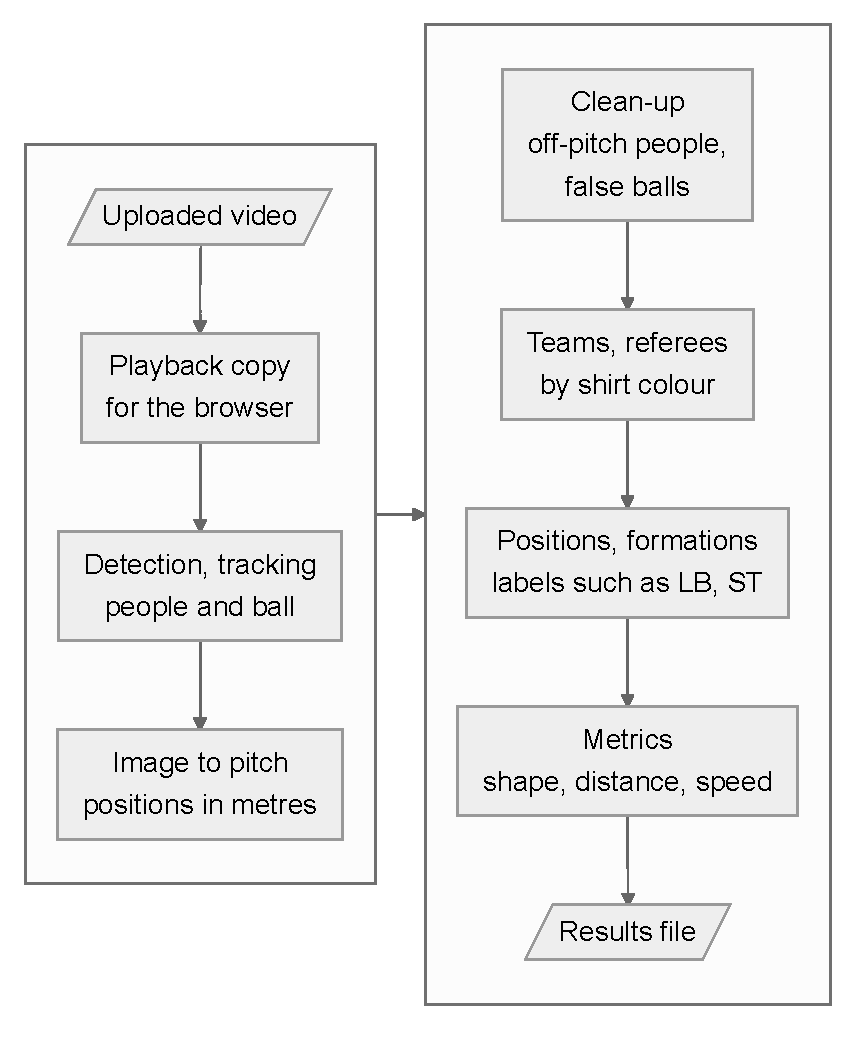
\includegraphics[width=0.65\textwidth]{pipeline}
	\caption{The stages of the analysis pipeline}
	\label{fig:pipeline}
\end{figure}

\subsection{Video input}

The worker first re-encodes the upload into an H.264 copy that every browser can play, with exactly one output frame per input frame so the overlays stay in sync. All later stages read this copy rather than the original: the two halves were encoded in AV1, and OpenCV failed with ``Corrupt frame detected'' whenever it had to jump within them. Frames are read in batches of four, so even a full half never sits in memory. Standard mode analyses every second frame of a 25\,fps video; for 50\,fps video the step is doubled, so every video is analysed at the same rate per second of play.

\subsection{Detection and tracking}

YOLOv8~\cite{yolov8}, with weights trained on broadcast football~\cite{roboflowsports}, finds players, goalkeepers, referees and the ball in each analysed frame. ByteTrack~\cite{bytetrack} links the people into tracks with stable IDs; it predicts each track's next position and matches new detections to it, including low-confidence detections of partly hidden players. The ball is not tracked this way, because it moves too fast; the five most likely ball candidates per frame are kept and the real one is chosen later.

\subsection{From the image to the pitch}

To measure in metres, each player's foot point is converted from image pixels to pitch coordinates. The pitch is a plane, and the mapping between a plane and its image is a homography~\cite{hartley}, a $3 \times 3$ matrix $H$:
\begin{equation}
	(X, Y, W)^T = H \, (x, y, 1)^T, \qquad \text{pitch point} = (X/W,\; Y/W).
\end{equation}
A second YOLOv8 model finds up to 32 known pitch landmarks in the image, such as the corners of the penalty areas (\autoref{fig:keypoints}). Their real positions on a $105 \times 68$\,m pitch are known, so $H$ can be fitted from them with RANSAC~\cite{ransac}, which ignores single wrongly detected landmarks. Because the camera pans and zooms, a new $H$ is fitted every few frames.

\begin{figure}[H]
	\centering
	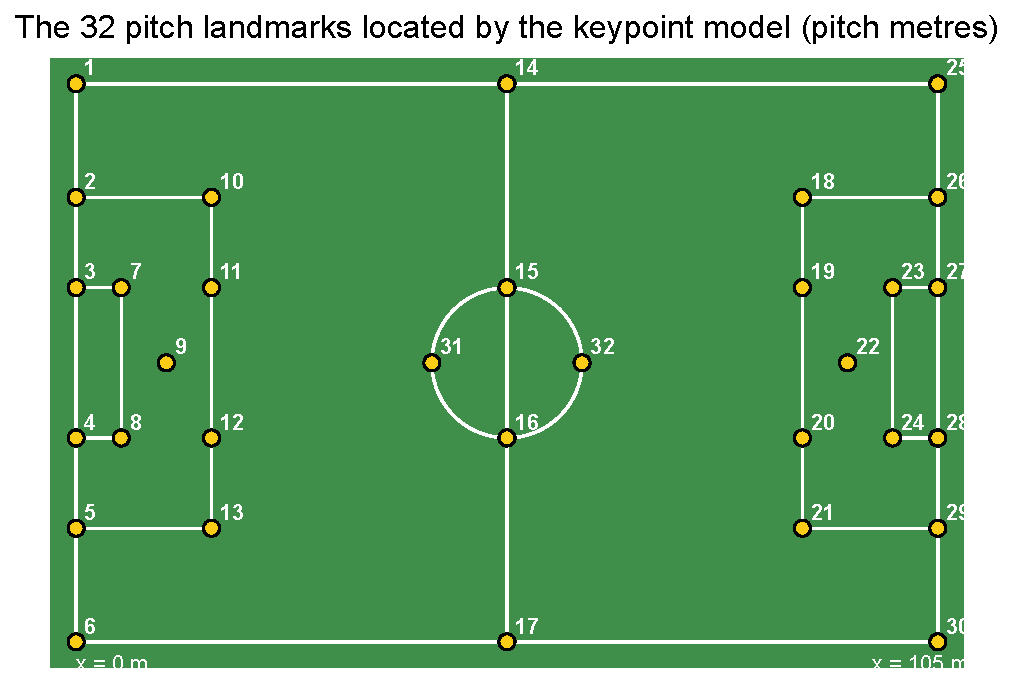
\includegraphics[width=0.85\textwidth]{pitch_keypoints}
	\caption{The 32 pitch landmarks}
	\label{fig:keypoints}
\end{figure}

Each fit is made on its own, so neighbouring fits can disagree slightly even though the real camera moved smoothly. On the first full half this made all movement paths jump across the video whenever a new fit arrived. The worker therefore smooths the camera model: it follows where four fixed points of the picture land on the pitch, smooths those positions over 1.5 seconds with a running median, and rebuilds $H$ from them. This cut the large jumps by about three quarters (\autoref{fig:camera-wobble}) while moving player positions by a median of only 0.16\,m.

\begin{figure}[H]
	\centering
	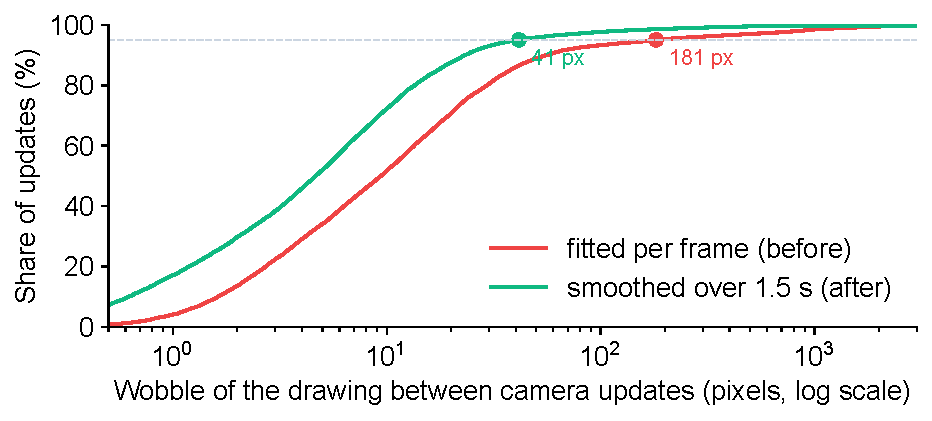
\includegraphics[width=0.9\textwidth]{camera_wobble}
	\caption{Jumps of the camera model before and after smoothing}
	\label{fig:camera-wobble}
\end{figure}

\subsection{Clean-up}
\label{sec:cleanup}

During stoppages a full half showed the touchline, where substitutes and staff stand, and spare balls lying beside it. With positions in metres both are easy to remove. A person whose usual (median) position is more than 0.5\,m outside the pitch lines is not part of the game and is removed; deciding over the whole track keeps a player who steps out for a throw-in. For the ball, the candidate closest to where the ball was a moment ago is kept, as long as the ball could have got there (no shot is faster than about 40\,m/s); candidates off the pitch and on the penalty spots are ignored when the path restarts. On the first half this removed 258 tracks of sideline people, and the share of ball positions off the pitch fell from 12\,\% to 0. \autoref{fig:ball-candidates} shows a stoppage after a goal, in which the old rule placed the ball on a spare ball beyond the far touchline in 344 of 375 frames.

\begin{figure}[H]
	\centering
	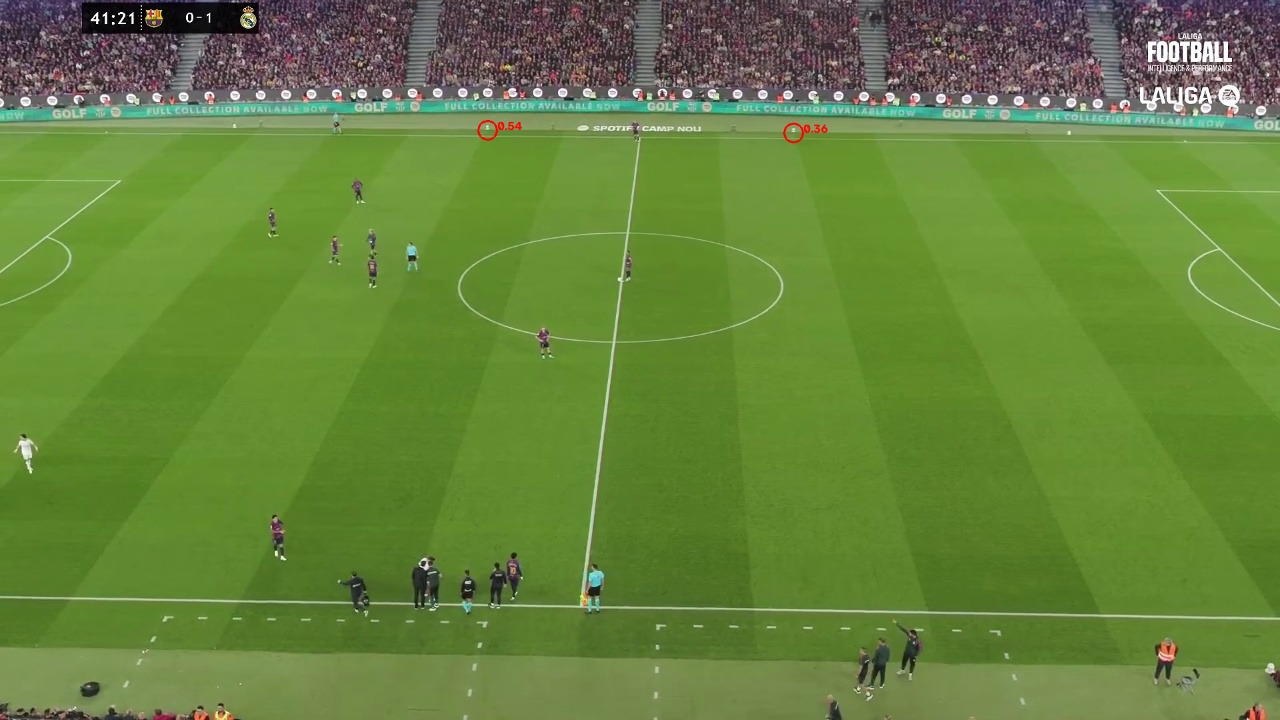
\includegraphics[width=\textwidth]{ball_candidates}
	\caption{Ball candidates during a stoppage: the two red circles are spare balls behind the far touchline, which the old rule took for the match ball}
	\label{fig:ball-candidates}
\end{figure}

\subsection{Teams and referees}

Players are split into teams by shirt colour. For each track, the torso region of up to ten detections is cropped, the grass colour measured around the player is removed, and the remaining pixels give the shirt colour in the CIE Lab colour space~\cite{opencvlab}. K-Means~\cite{kmeans} then splits the tracks into two teams. Goalkeepers wear a different kit, so they join the team whose players are closest to them.

The detector often called the main referee a player, and he then joined a team. The referee kit colour is therefore learned from the tracks the model does call referees (usually the assistants), and a ``player'' whose shirt is much closer to that colour than to either team colour becomes a referee. To choose ``much closer'', I ranked the candidate tracks and looked at a crop of each: below a ratio of about 0.65 almost all were officials, and from 0.68 white Real Madrid players appeared. A goalkeeper is only checked if he stands outside both penalty areas, because goalkeepers also wear a colour unlike both teams.

\subsection{Joining tracks and position labels}
\label{sec:positions}

ByteTrack starts a new track whenever it loses a player for two seconds, and the first half produced 1,423 tracks for about 25 people. Tracks that end and start again within five seconds, nearby and with the same team, are joined with the Hungarian algorithm~\cite{hungarian}, which left 555. Fewer is not possible with one camera: a player who is out of view for half a minute cannot be recognised, because all players of a team wear the same kit and shirt numbers are only a few pixels tall.

Instead of track numbers, players are therefore labelled by position. The formation step (below) assigns every visible player to a slot of the team's formation, such as LB or ST; these slots become the labels, smoothed over time so that they do not flicker. A label follows the position, not the person: if two players swap sides, their labels swap too.

\subsection{Formations}

A formation cannot be seen in a single frame, so the average positions of a team's outfield players are computed over 5-second windows, scaled to a unit square and compared with nine formation templates (\autoref{fig:templates}). The cost of a template is the mean distance between players and slots under the best one-to-one assignment, found with the Hungarian algorithm (\autoref{fig:matching}). A new formation is only accepted when it fits clearly better than the current one and has lasted 20 seconds; without this rule the first half reported 282 formation changes instead of 14.

\begin{figure}[H]
	\centering
	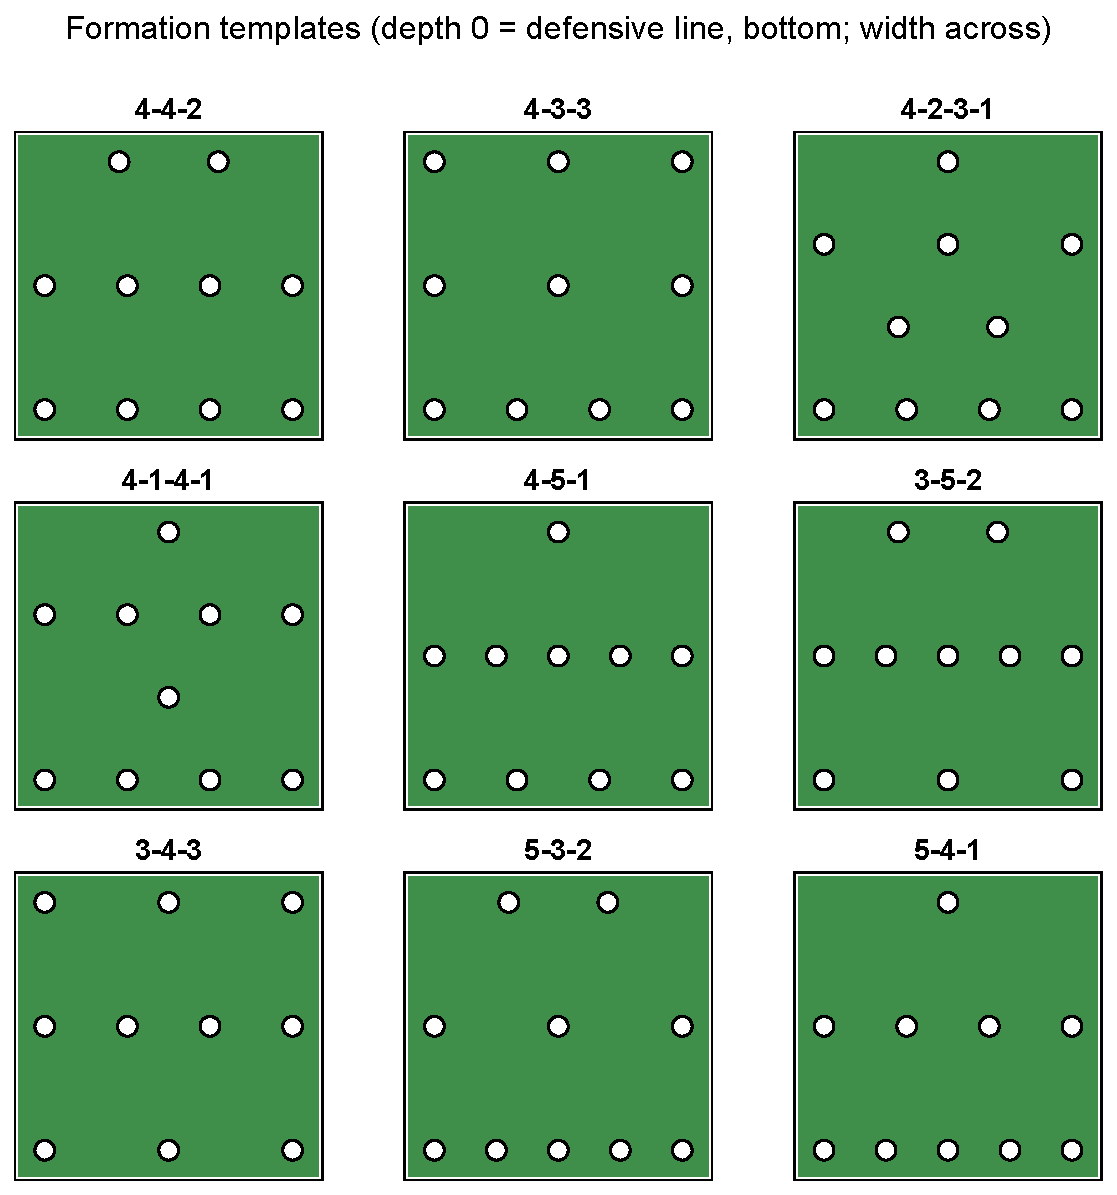
\includegraphics[width=0.62\textwidth]{formation_templates}
	\caption{The nine formation templates}
	\label{fig:templates}
\end{figure}

\begin{figure}[H]
	\centering
	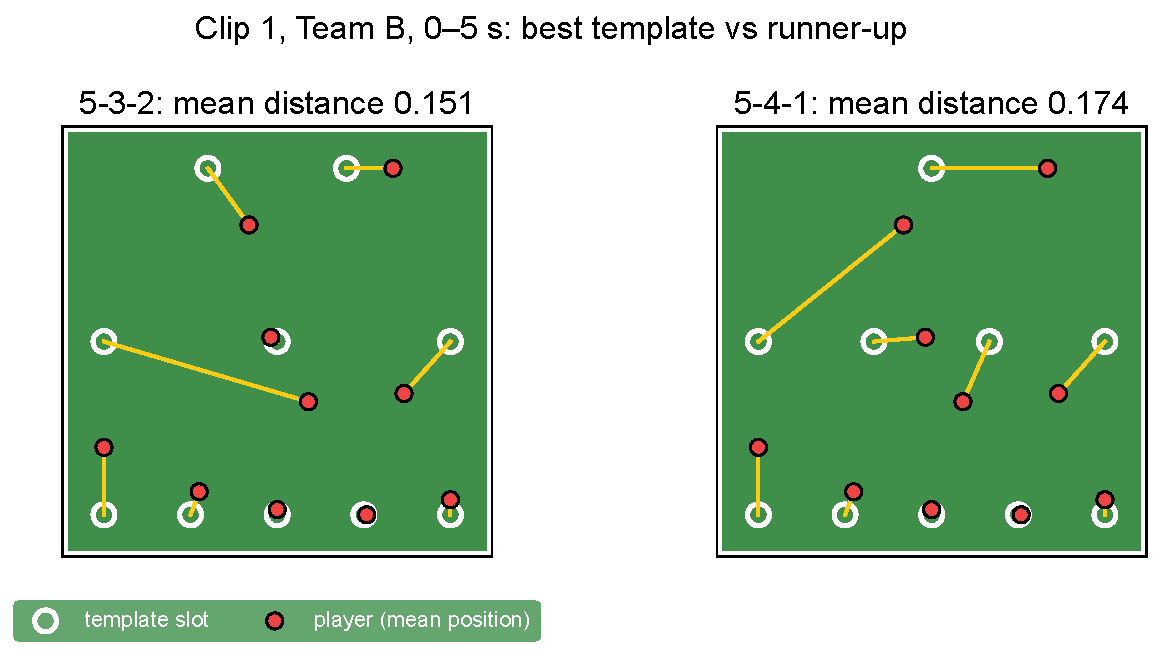
\includegraphics[width=\textwidth]{formation_matching}
	\caption{Matching one window of a team to the best template and the runner-up}
	\label{fig:matching}
\end{figure}

\subsection{Metrics}
\label{sec:metrics}

The worker determines each team’s compactness (the area of the convex hull of its outfield players), width and depth per frame from the smoothed positions, and the distance travelled by each position, how long it was in view, the average speed, and a heatmap for every position. Any steps with speeds greater than 12\,m/s will be considered as tracking errors and are ignored. The top speed is the best average over one second versus the fastest single step; an earlier version incorrectly reported 39.6\,km/h on one clip due to a single displaced position being considered a sprint.
